\documentclass[10pt,twocolumn,letterpaper]{article}

\usepackage{cvm}
\usepackage{times}
\usepackage{epsfig}
\usepackage{graphicx}
\usepackage{amsmath}
\usepackage{amssymb}
\usepackage{subcaption}


% Include other packages here, before hyperref.

% If you comment hyperref and then uncomment it, you should delete
% egpaper.aux before re-running latex.  (Or just hit 'q' on the first latex
% run, let it finish, and you should be clear).
\usepackage[pagebackref=true,breaklinks=true,letterpaper=true,colorlinks,bookmarks=false]{hyperref}


% \cvmfinalcopy % *** Uncomment this line for the final submission

\def\cvmPaperID{****} % *** Enter the cvm Paper ID here
\def\httilde{\mbox{\tt\raisebox{-.5ex}{\symbol{126}}}}

% Pages are numbered in submission mode, and unnumbered in camera-ready
\ifcvmfinal\pagestyle{empty}\fi
\begin{document}

%%%%%%%%% TITLE
\title{Efficient sketch-based character modelling with primitive deformer and shape generator}

\author{First Author\\
Institution1\\
Institution1 address\\
{\tt\small firstauthor@i1.org}
% For a paper whose authors are all at the same institution,
% omit the following lines up until the closing ``}''.
% Additional authors and addresses can be added with ``\and'',
% just like the second author.
% To save space, use either the email address or home page, not both
\and
Second Author\\
Institution2\\
First line of institution2 address\\
{\small\url{http://www.author.org/~second}}
}

\maketitle
% \thispagestyle{empty}

%%%%%%%%% ABSTRACT
\begin{abstract}
This paper proposes a new sketch-guided and ODE-driven character modelling technique. Our system consists of two main components: primitive deformer and detail generator. With such a technique, we first draw 2D silhouette contours of a character model. Then, we select proper primitives and align them with the corresponding silhouette contours. After that, we develop a sketch-guided and ODE-driven primitive deformer. It uses ODE-based deformations to deform the primitives to exactly match the generated 2D silhouette contours in one view plane and obtain a base mesh of a character model consisting of deformed primitives. In order to add various 3D details, we develop a local shape generator which uses sketches in different view planes to define a local shape and employs ODE-driven deformations to create a local surface passing through all the sketches. \\
The experimental results demonstrate that our proposed approach can create 3D character models with 3D details from 2D sketches easily, quickly and precisely.
\\
\end{abstract}

%%%%%%%%% BODY TEXT
\section{Introduction}
\begin{itemize}
  \item[$\bullet$] We develop an efficient sketch-guided and ODE-driven primitive deformer to create a base mesh. It can deform primitives to exactly match the generated silhouette contours. Compared to the existing methods, it automates shape manipulation, avoids tedious manual operations, can deform primitives to match the generated silhouette contours quickly, and is powerful in achieving different shapes of a same primitive.
  \item[$\bullet$] We develop a detail generator to add 3D details to the base mesh. Our proposed sketch-guided and ODE-driven local shape creator can create a new local shape to match user's drawn sketches in different views quickly. The image-based detail generator can automatically generate fine details from 2D images. 
  \item[$\bullet$] Our character modelling system provide editing operations, support users to manipulate the control curves the draw in the creation stage and adding more control curves after the surface has been created. With our developed system, 3D character models with 3D details can be created easily and efficiently.
\end{itemize}
The rest of the paper is organised as follows. The previous related work is briefly reviewed in Section \ref{related_work}. The system overview of our proposed approach is presented in Section \ref{system_overview}. Primitive deformer is examined in Section \ref{primitive_deformer}, and Detail generator is investigated in Section \ref{detail_generator}. Finally, the conclusions and future work are discussed in Section \ref{conclusions_and_future_work}. 


\section{Related Work}\label{related_work}

\subsection{Inflation Technology}
Over the past two decades, sketch-based-modelling (SBM) has been widely studied in the computer graphic research community. Several research based systems have been proposed to generate organic models. The surface inflation technique extrudes the polygonal mesh from the skeleton outwards do a good job in modelling stuffed toys. One trend is to inflate freeform surfaces to create simple stuffed animals and other rotund objects in a sketch-based modelling fashion, such as \cite{igarashi1999teddy, Karpenko:2006:SFS:1141911.1141928, nealen2007fibermesh}. The Teddy system \cite{igarashi1999teddy} is the pioneer, it takes closed curves as inputs and find their cordial axes as spline, then wrap the splines with the polygonal mesh. Later, FiberMesh\cite{nealen2007fibermesh} enriched the editing operations for the inflating base mesh. FiberMesh also presents two types of the control curves: smooth and sharp. A smooth curve constrains the surface to be smooth across it, while a sharp curve only places positional constraints with C0 continuity. Sharp control curves appears when operations like cutting, extrusion and tunnel take place. Sharp control curves also serves the creation of creases on surface. However, FiberMesh \cite{nealen2007fibermesh} doesn't allow users to specify the ROI.Based on the study from William\cite{williams1997stochastic}, the SmoothSketch system addressed the problem of T-junction and cusp, which Teddy fails to solve.
%-------------------------------------------------------------------------
\subsection{Primitive Technology}
Unlike the inflating systems, primitives-based systems deconstruct the modelling task as a process of creating a certain set of geometry primitives and further editing on the primitives. The idea of assembling simple geometry primitives to form 3D models is very common in CSG(constructive solid geometry) modelling, related researches including \cite{shtof2013geosemantic,chen20133}. Shtof et.al \cite{shtof2013geosemantic} introduces a snapping method which helps determining the position and core parameters of several simple geometry primitives. In \cite{chen20133}, the authors provides tools for generating a cylinder from only 3 strokes: the first two strokes define the 2D profile and the last stroke defines the axis along which the profile curve will sweep. Copies of the profile are not only perpendicularly aligned to the axis, but also resized to snap to the input outlines. However their work is only for man-made objects which simple sweeping surface can meet the quality requirements of the shapes. Structured Annotations for 2D-to-3D Modelling \cite{gingold2009structured}, on the other hand, focus on organic modelling. It is a system using two sets of the primitives, one is generalized cylinders, created by the input of a single open sketch stroke representing the spline, and then modified by using simple gestures such as tilt, scale local radius, rotate symmetrical plane, and change cap size; the other primitive is ellipsoid, generated according to the drawn closed ellipse sketch stroke. As the system's name indicates, there are a set pf annotation tools to further editing the surface shape using the annotations such as same-lengths, same angles, alignment and mirror symmetry. 

\subsection{Mesh editing}
A universal disadvantage of above systems is features provided are limited it was not suited to modelling complex and production ready models. This is partly due to their limitations in mesh editing operations, so several sketch-based editing methods have been development to help to improve the performance of sketch-based modelling system. One group of sketch-based editing methods \cite{draper2003gestural, kho2005sketching} treats individual sketch curve as the reference for deformations like bending. Take the \cite{kho2005sketching} for example, user will draw a first curve as a reference curve to both set the ROI (region of interest) and be a controlling 'skeleton', and a new sketch curve indicating the desired deformation of the reference curve. Then mapping the reference curve to the second curve, the ROI will be deformed. These methods are very useful for simple keyframe animation, but for more small-scaled shape's editing task, studies like \cite{lipman2004differential,nealen2007sketch,SBM:SBM07:023-030} are more suitable. These studies take mesh's contours (depend on the viewplan at the time of editing operation is happening) as reference curves, and the newly sketched curves indicating the new positions that the ROI of mesh should be reconstructed to. As they aiming at maintaining the local geometrical details, Laplacian coordinates and correspondingly laplacian surface editing technology are implemented to preserving the features. 

\section{System Overview}\label{system_overview}
Based on our proposed approach, we have developed a modelling system which is composed of two main components: primitive deformer and detail generator. The primitive deformer is used to deform primitives to exactly match user's generated 2D silhouette contours and create a rough base mesh. The detail generator consists of local shape creator and image-based detail generator. The local shape creator creates a new local shape from four different algorithms. They are local shape creation from: 1) two open silhouette contours in two different view planes, 2) one open and one closed silhouette contour in two different view planes, 3) two open and one closed silhouette contours in three different view planes, and 4) two closed curves. The image-based detail generator generates fine 3D details from 2D images automatically through the SFS algorithm.  
The modeling process using our developed system is demonstrated in Figure 1 where a 3D female warrior model is created. 
 
 \begin{figure}[t]
\begin{center}
%\fbox{\rule{0pt}{2in} \rule{0.9\linewidth}{0pt}}
 %  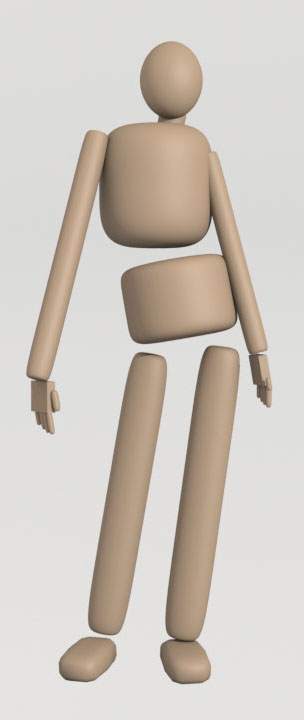
\includegraphics[width=0.7\linewidth]{./figure/primitives_before_deformation.jpg}\label{fig:long}
  \begin{subfigure}[!t]{0.32\linewidth}
       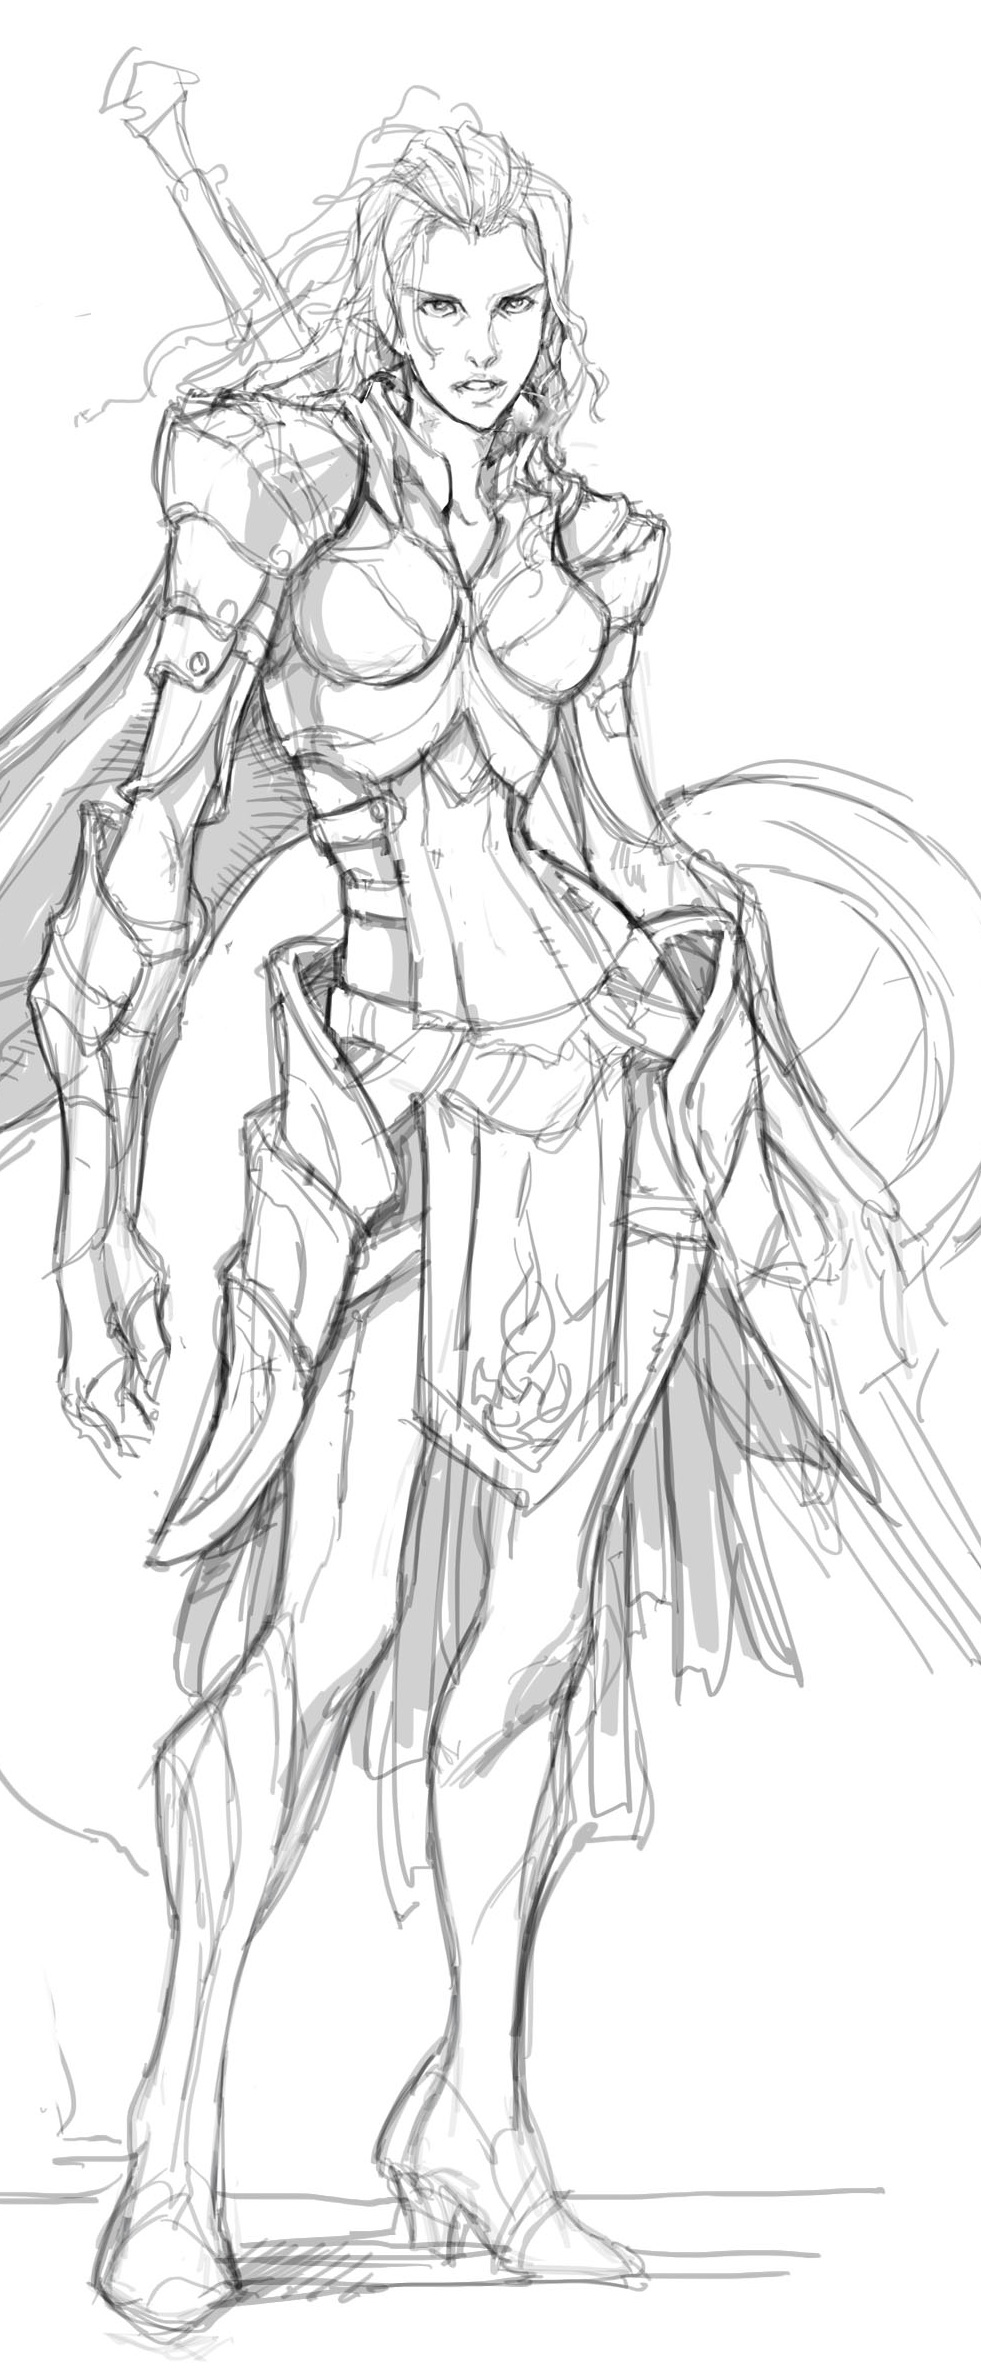
\includegraphics[height=2.3in]{./figure/female_warrior_original_sketch.jpg}
        \caption{}\label{fig:reference_image}
    \end{subfigure}
     \begin{subfigure}[!t]{0.32\linewidth}
       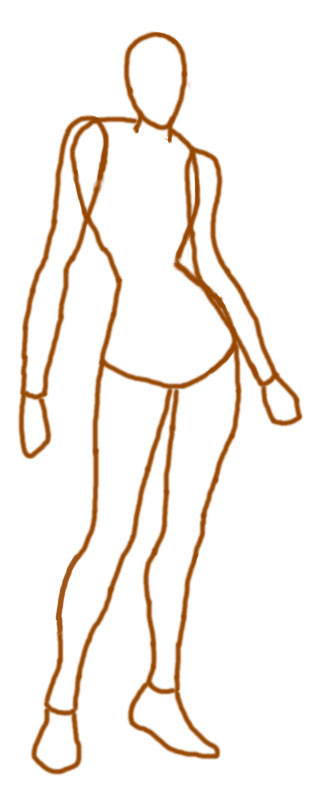
\includegraphics[height=2.3in]{./figure/female_warrior_extract_contour.jpg}
        \caption{}\label{fig:extract_contour}
    \end{subfigure}
 \begin{subfigure}[!t]{0.32\linewidth}
       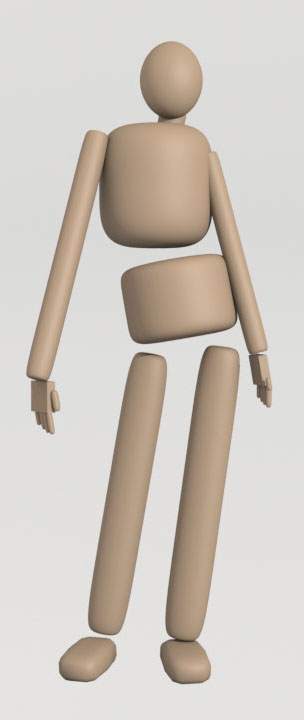
\includegraphics[height=2.3in]{./figure/primitives_before_deformation.jpg}
        \caption{}\label{fig:superellipsoid_primitives}
    \end{subfigure}
   % \hskip0.5em
    \begin{subfigure}[!t]{0.32\linewidth}
        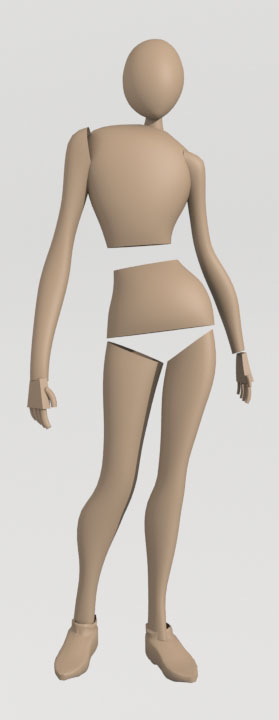
\includegraphics[height=2.3in]{./figure/primitives_after_deformation_without_blending.jpg}
        \caption{}\label{fig:primitives_after_deformation}
    \end{subfigure}
    \begin{subfigure}[!t]{0.32\linewidth}
        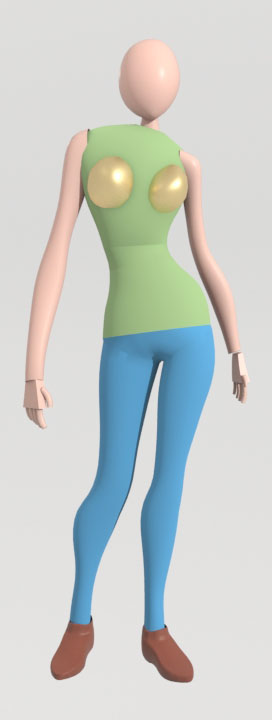
\includegraphics[height=2.3in]{./figure/primitives_after_deformation_and_lattice_with_breast.jpg}
        \caption{}\label{fig:blending_body_parts}
    \end{subfigure}
    \begin{subfigure}[!t]{0.32\linewidth}
        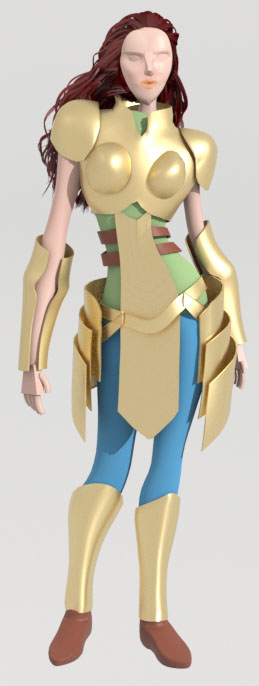
\includegraphics[height=2.3in]{./figure/final_shot.jpg}
        \caption{}\label{fig:final_shot}
    \end{subfigure}
\end{center}
   \caption{Quick creation of a 3D female warrior model: (a) 2D female warrior sketch, (b) 2D silhouette contours, (c) base mesh without primitive deformations, (d) base mesh by deforming primitives to match generated 2D silhouette contours or adding local shapes created from 2D silhouette contours, (e) base mesh by adding blending surfaces to smoothly connect deformed primitives, (f) detail generation through local shape creation and shape from shading (Sketch by � EngKit Leong) 
  }
\label{fig:system_overview}
\end{figure}

First, 2D character silhouette contours are generated. Users can draw their own silhouette contours directly or input their selected sketches into our developed system. If the selected sketches are input into our developed system, a further process may be required to extract the 2D silhouette contours from the input sketches. For the example demonstrated in Figure \ref{fig:system_overview}, a 2D female warrior sketch shown in Figure \ref{fig:system_overview}\subref{fig:reference_image} is input. Then, users can extract 2D silhouette contours from the input sketch as shown in Figure \ref{fig:system_overview}\subref{fig:extract_contour}. After that, proper primitives are selected and placed to align with the corresponding silhouette contours through purely geometric transformations as shown in Figure \ref{fig:system_overview}\subref{fig:superellipsoid_primitives}. Since the silhouette contours of the primitives do not match the generated 2D silhouette contours of the 2D female warrior, the primitive deformer developed from sketch-guided and ODE driven deformations described in Section 4 is applied to deform the primitives to exactly match the corresponding 2D silhouette contours and create a rough 3D base mesh depicted in Figure \ref{fig:system_overview}\subref{fig:primitives_after_deformation}. 
Once a 3D base mesh model is obtained, the detail generator described in Section 5 is employed to add 3D details to the 3D base mesh. First, the local shape creator developed in Subsection 5.2 is used to add local shapes and smoothly connect primitives together as demonstrated in Figure \ref{fig:system_overview}\subref{fig:blending_body_parts}. After that, we want to add fine details such as a dragon to the female warrior model. Since creating fine 3D details is not an easy task, we apply the image-based detail generator described in Subsection 5.3 to achieve the complicated 3D details shown in Figure \ref{fig:system_overview}\subref{fig:final_shot}.
In the following two sections, we will introduce in detail the primitive deformer and the detail generator, respectively. Some examples will be presented to demonstrate their applications.

\section{Primitive deformer}\label{primitive_deformer}
As shown in Figure \ref{fig:system_overview}\subref{fig:superellipsoid_primitives}, the base mesh of the female warrior without primitive deformations cannot exactly match the generated 2D silhouette contours of the female warrior. In order to tackle this problem, in this section, we develop a primitive deformer. In the subsections below, we first introduce the interface of the primitive deformer in Subsection \ref{user_interface_of_primitive_deformer}. Then, we discuss the algorithm of the primitive deformer in Subsection \label{algorithm_of_primitive_deformer}.
\subsection{User interface of primitive deformer} \label{user_interface_of_primitive_deformer}
The user interface of our developed primitive deformer uses four windows. The upper left window is used to display 3D base mesh without primitive deformations in the front view. The upper right window is used to display primitives and the user-drawn 2D silhouette contours for these primitives. If required, the user can edit the generated 2D silhouette contours in the upper right window. The deformed primitives are shown in the bottom windows where the left is from the front view and the right is from the side view. 
Taking the left leg of the female warrior shown in Figure 1(c) as an example, the primitive of the left leg is shown in the upper left window. It and the user-drawn 2D silhouette contours are depicted in the upper right window. Our proposed primitive deformer described in Subsection 4.2 deforms the primitives of the 3D base mesh to exactly match the generated 2D silhouette contours and create a deformed 3D base mesh with primitive deformations, and depicted the deformed 3D base mesh in bottom windows. 
\subsection{Algorithm of primitive deformer}\label{algorithm_of_primitive_deformer}
After 3D primitives have been placed and aligned with the generated 2D silhouette contours, these 3D primitives should be deformed so that their 2D silhouette contours can match the generated 2D silhouette contours exactly. Here we use the example shown in Figure 3 to demonstrate the algorithm of our proposed primitive deformer and how it deforms a 3D primitive to match the 2D silhouette contours. 
Figure 3(a) depicts an arm model of the female warrior which is represented with a cylinder. The 2D silhouette contour to be matched is also shown in the image. Figure 3(b) shows how the cylinder is deformed with the algorithm developed below to match the 2D silhouette contour exactly. 
To tackle the above problem, we propose a sketch-guided and ODE-drive primitive deformer. It is developed from a simplified version of the Euler-Lagrange PDE (partial differential equation) which is widely used in physically-based surface deformations and briefly introduced below.
As discussed in \cite{botsch2008linear}, the main requirement for physically-based surface deformations is an elastic energy which considers locally stretching for solid objects plus bending for two-manifold surfaces called thin-shells. When a surface $\mathbb{S} \subset \mathbb{R}^3$ parameterized by a function $\mathbf{P(u,v)}: \Omega \subset  \mathbb{R}^2 \mapsto \mathbb{S} \subset \mathbb{R}^3 $is deformed to a new shape $\mathbb{S'}$ through adding a displacement vector $\mathbf{d(u,v)}$ to each point $\mathbf{P(u,v)}$, the change of the first and second fundamental $I(u,v),\Pi(u,v) \in \mathbb{R}^{2\times2}$,forms in differential geometry \cite{do2017differential} yields a measure of stretching and bending descried by \cite{terzopoulos1987elastically}
\begin{equation}
E_{shell}(S') = \int_{\Omega}k_s\|I'-I\|_F^2+k_b\|\Pi'-\Pi\|_F^2 dudv \label{energy}
\end{equation}
Where ,$I'$,$\Pi'$ are the first and second fundamental forms of the surface $\mathbf{S'}$,  $ \| . \|$ indicates a (weighted) Frobenius norm, and the stiffness parameters $k_s$  and $k_b$ are used to control the resistance to stretching and bending. 
Generating a new deformed surface requires the minimization of the above equation which is non-linear and computationally too expensive for interactive applications. In order to avoid the nonlinear minimization, the change of the first and second fundamental forms is replaced by the first and second order partial derivatives of the displacement function $\mathbf{d(u,v)}$ (Celniker, 1991), (Welch, 1992) , i. e.,   
\begin{equation}
\tilde{E}_{shell}(d) = \int_{\Omega}k_s(\|d_u\|^2+\|d_v\|^2)+k_b(\|d_{uu}\|^2+2\|d_{uv}\|+\|d_{vv}\|^2) dudv \label{energydiffgeo}
\end{equation}
where $d_x=\frac{\partial}{\partial{x}}$ and $d_{xy}=\frac{\partial^2}{\partial{x}\partial{y}}$ .
The minimization of the above equation can be obtained by applying variational calculus which leads to the following Euler-Lagrange PDE
\begin{equation}
-k_s\triangle d+k_b\triangle^2d=0
\label{lagrange}
\end{equation}
where $\triangle$ and $\triangle^2$ are the Laplacian and the bi-Laplacian operator, respectively.
\begin{equation}
\begin{aligned}
\triangle d &=div\nabla d=d_{uu}+d_{vv} \\
\triangle^2d=\triangle(\triangle d) &=d_{uuuu}+2d_{uuvv}+d_{vvvv}
\label{laplacianoperator}
\end{aligned}
\end{equation}
Using the generated 2D silhouette contours shown in Figure \ref{fig:silhouette} to change the shape of the primitive can be transformed into generation of a sweeping surface which passes through the two generated 2D silhouette contours. The generator creating the sweeping surface is a curve of the parametric variable  only, and the two silhouette contours are trajectories. If Equation \eqref{lagrange} is used to describe the generator, the parametric variable  in Equation \eqref{lagrange} drops, and we have  $d_{vv}=0$ and $d_{vvvv}=0$. Substituting  and  into Equation \eqref{lagrange}, we obtain the following simplified version of the Euler-Lagrange PDE \eqref{lagrange}which is actually a vector-valued ordinary differential equation
\begin{equation}
k_b\frac{\partial^4d}{\partial u^4}-k_s\frac{\partial^2 d}{\partial u^2}=0
\label{ODE}
\end{equation}
As pointed out in \cite{chaudhry2013shape} and \cite{chaudhry2015dynamic} , the finite difference solution of ordinary differential equations is very efficient, we here investigate such a numerical solution of Equation \eqref{laplacianoperator}.
\begin{figure}[h!tb]
	\begin{center}
	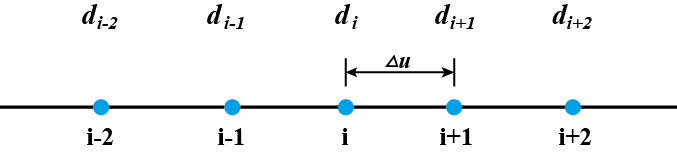
\includegraphics[width=0.9\columnwidth]{./figure/FDM.png}
	\end{center}
	\caption{Typical node i  for the finite difference approximations of derivatives}
	\label{fig:fdm}
\end{figure}
For a typical node  shown in Figure \ref{fig:fdm}, the central finite difference approximations of the second and fourth order derivatives can be written as \cite{chaudhry2013shape}
\begin{equation}
\begin{split}
\frac{\partial^2d}{\partial u^2}|_i &=\frac{1}{\triangle u^2}(d_{i+1}-2d_i+d_{i+1}) \\
\frac{\partial^4d}{\partial u^4}|_i &=\frac{1}{\triangle u^4}[6d_i-4(d_{i-1}+d_{i+1})+d_{i-2}+d_{i+2}]
\label{FDM}
\end{split}
\end{equation}
Introducing Equation \eqref{FDM} into Equation \eqref{ODE}, the following finite difference equation at the representative node $i$ can be written as:
\begin{equation}
\begin{split}
(6k_b+2k_sh^2)d_i+k_bd_{i-2}+k_bd_{i+2} \\
-(4k_b+k_sh^2)d_{i-1}-(4k_b+k_sh^2)d_{i+1}=0
\end{split}
\label{odefdm}
\end{equation}
For character models, the 3D shape defined by two silhouette contours is closed in the parametric direction u as indicated in Figure \ref{fig:FDMnode}(b). Therefore, we can extract some closed curves each of which passes through the two corresponding points on the two silhouette contours. Taking the silhouette contours in Figure 3(b) as an example, we find two corresponding points $\mathbf{c_{13}}$ and $\mathbf{c_{23}}$ on the original silhouette contours $\mathbf{c_1}$ and $\mathbf{c_2}$, and two corresponding points $\mathbf{c'_{13}}$ and $\mathbf{c'_{23}}$ on the deformed silhouette contours $\mathbf{c'_1}$ and $\mathbf{c'_2}$ as shown in Figure \ref{fig:FDMnode}(b). Then we extract a closed curve $\mathbf{c(u)}$ passing through the two corresponding points $\mathbf{c_{13}}$ and $\mathbf{c_{23}}$ from the 3D model in Figure \ref{fig:FDMnode}(a) and depicted it as a dashed curve in Figure \ref{fig:FDMnode}(b). Assuming that the deformed shape of the closed curve $\mathbf{c(u)}$ is $\mathbf{c'(u)}$, the displacement difference between the original closed curve and deformed closed curve is $\mathbf{d(u)=c'(u)-c(u)}$. Our task is to find the displacement difference $\mathbf{d(u)}$ and generate the deformed curve $\mathbf{c'(u)=d(u)+c(u)}$.
\begin{figure}[h!tb]
	\begin{center}
	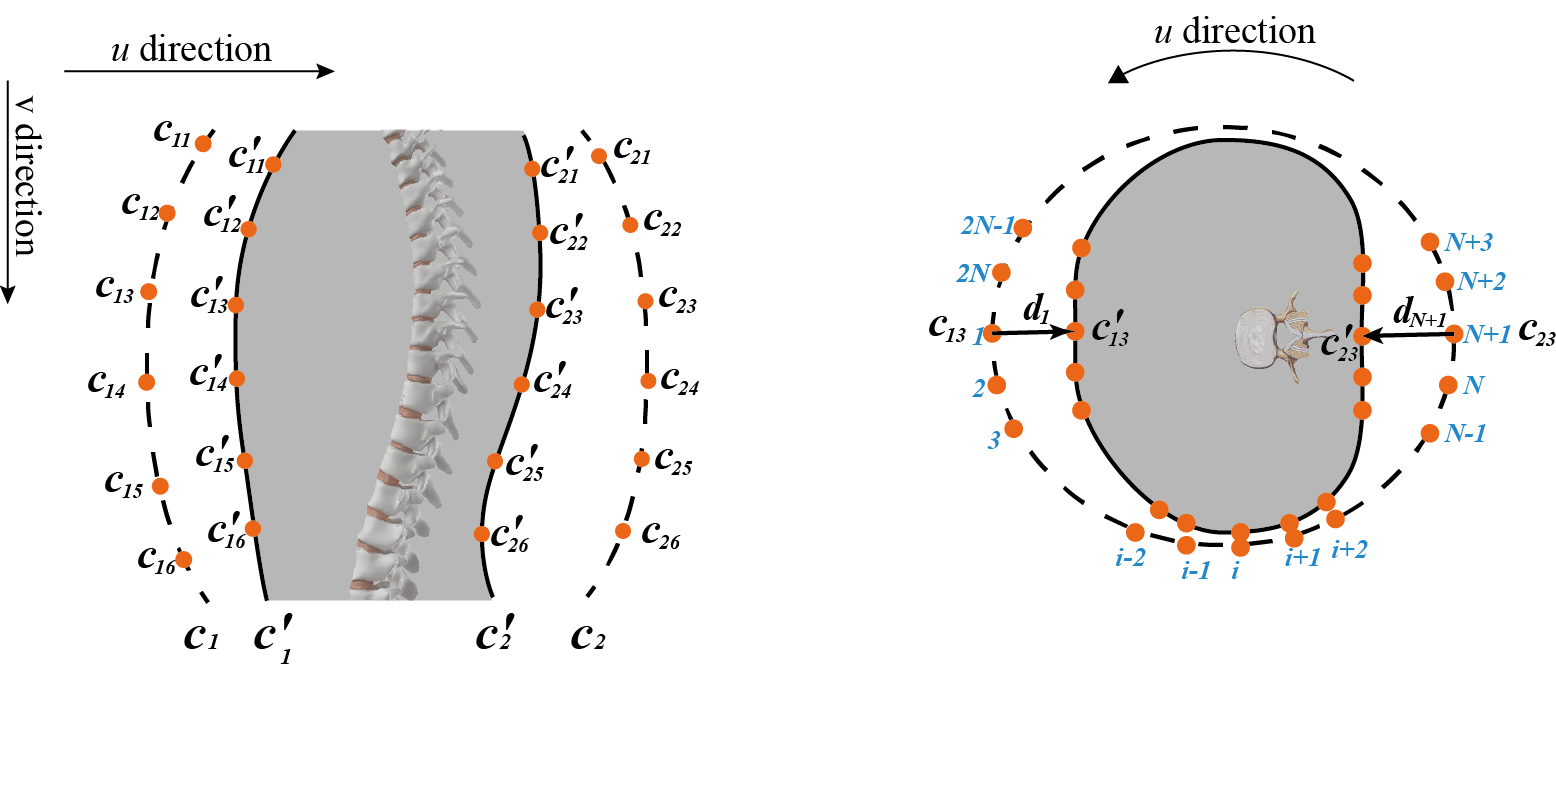
\includegraphics[width=0.9\columnwidth]{./figure/fdmnode.png}
	\end{center}
	\caption{Finite difference nodes for local shape manipulation from sketches in the same view plane}
	\label{fig:FDMnode}
\end{figure}
In order to use the finite difference method to find the displacement difference $\mathbf{d(u)}$, we uniformly divide the closed curve into $2N$ equal interval as indicated in Figure \ref{fig:FDMnode}. The displacement difference at node 1 and node $\mathbf{N}$ is known, i. e. $\mathbf{d_1=c'_{13}-c_{13}}$ and $\mathbf{d_{N+1}=c'_{23}-c_{23}}$. 
When we write the finite difference equations for the nodes 2, 3, $2N-1$ and $2N$, the node 1 will be involved, and we have  $\mathbf{d_1=c'_{13}-c_{13}}$. The finite difference equations at these points can be derived from Equation \eqref{odefdm}. Substituting  $\mathbf{d_1=c'_{13}-c_{13}}$ into these equations, we obtain the finite difference equations for the nodes 2, 3, $2N-1$ and $2N$%, and present them in Appendix A. 
When we write the finite difference equations for the nodes $N-1$,$N$, $N+2$ and $N+3$, the node $N+1$ will be involved, and we have $\mathbf{d_{N+1}=c'_{23}-c_{23}}$. Once again, the finite difference equations at these points can be derived from Equation \eqref{odefdm}. Substituting $\mathbf{d_{N+1}=c'_{23}-c_{23}}$ into these equations, we obtain the finite difference equations for the nodes N-1, N, N+2 and N+3%, and present them in Appendix A as well. 
For all other nodes 3, 4, 5,\ldots, $N-3$ , $N-2$ and $N+4$,$N+5$ ,\ldots, $2N-3$, $2N-2$, the finite difference equations are the same as Equation \eqref{odefdm}. For these nodes, there are $2N-5$ finite difference equations. Plus the 8 finite difference equations at node 2, 3, $N-1$ , $N$ , $N+2$ , $N+3$ , $2N-1$ and $2N$, we get  $2N-2$linear algebra equations which can be solved to determine the  unknown constants $\mathbf{d_2}$, $\mathbf{d_3}$ , \ldots,$\mathbf{d_{N-1}}$, $\mathbf{d_{N}}$ , $\mathbf{d_{N+2}}$ , $\mathbf{d_{N+3}}$ ,\ldots, $\mathbf{d_{2N-1}}$, and $\mathbf{d_{2N}}$. Adding the $\mathbf{d_i}$ ( $i=1,2,\ldots,2N-1,2N$) to the original curve $\mathbf{c(u)}$, we obtain the deformed curve $\mathbf{c'(u)}$, and depict it as a solid curve in Figure \ref{fig:FDMnode}(b). Repeating the above operations for all other points on the two silhouette contours, we obtain all deformed curves. These curves describe a new 3D deformed shape.\\
Taking a finger shown in Figure 5(c) as an example, the left image shows the silhouette contours. It is used deform a cylinder into the middle 3D model (the second image from the left). The cross-section shapes of the finger model are depicted in the third image from the left. The rightmost image shows the five finger models created with the above method.\\
With the primitive deformer developed above, we deform the primitive of the 3D base mesh shown in Figure 1(c), obtain a deformed 3D base mesh, and depicted it in Figure 1(d). We have also deformed the primitives to match the silhouette contours of the Knight sketches shown in Figure 6(a), and obtain the deformed 3D base mesh of the knight model shown in Figure 6(b). It is clear that deformed primitives have matched the generated 2D silhouette contours exactly. 

Figure \ref{fig:arm} depicts an arm model which is represented with a generalized cylinder. Figure \ref{fig:arm}b shows the generated 2D silhouette contours of the arm and the generalized cylinder. Figure \ref{fig:arm}c shows after deforming the generalized cylinder, its 2D silhouette contours match generated 2D silhouette contours of the arm exactly. Since the silhouettes only define the shape on one dimension, we control the thickness of the arms via a ramp parameter (see fig.\ref{fig:arm} c,d)
\begin{figure}[!htb]
\centering
\begin{multicols}{2}
\resizebox{6.7cm}{3.4cm}{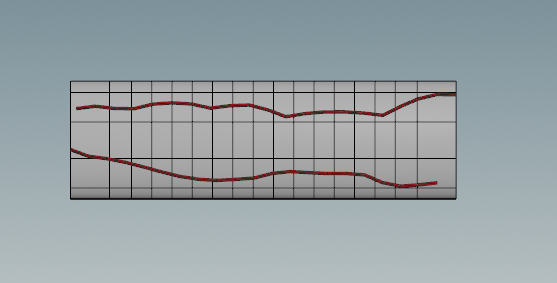
\includegraphics[width=\linewidth]{./figure/cylinder.png}}
\resizebox{6.7cm}{3.4cm}{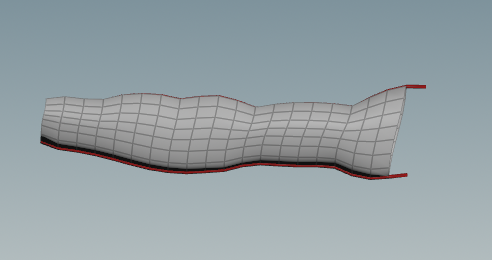
\includegraphics[width=\linewidth]{./figure/deformer.png}}
\end{multicols}
\begin{multicols}{2}
\resizebox{6.7cm}{3.4cm}{\includegraphics{./figure/ramp.png}}
\resizebox{6.7cm}{3.4cm}{\includegraphics{./figure/armtopview.png}}
\end{multicols}
\caption{Primitive deformer: a)male arm represented with a generalized cylinder, and the 2D silhouette contours of the male, b)deformed shape of the generalized cylinder c)the ramp parameter controlling the arm thickness d)arm on another view plane}
 \label{fig:arm}
\end{figure}
However, there are times when deforming from a uniform primitive is not ideal because the area of cross-section changes a lot. See Fig.\ref{fig:footfinger}(a). In such cases, we extract the cross-section first, scale them accordingly (Fig.\ref{fig:footfinger} (b)), and then using the same algorithm mentioned above to deform the pre-processed (Fig.\ref{fig:footfinger} (c)) primitives.
\begin{figure}[!htb]
\centering
\begin{multicols}{3}
\resizebox{4.3cm}{4.1cm}{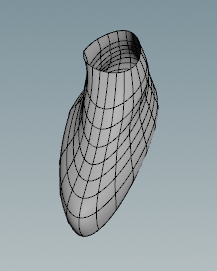
\includegraphics[width=\linewidth]{./figure/foot1.png}}
\resizebox{4.3cm}{4.1cm}{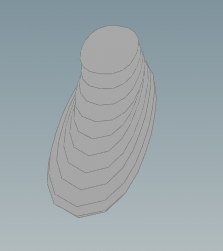
\includegraphics[width=\linewidth]{./figure/foot_scale_cross-section.png}}
\resizebox{4.3cm}{4.1cm}{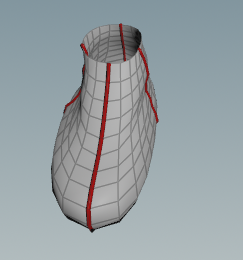
\includegraphics[width=\linewidth]{./figure/foot2.png}}
\end{multicols}
\begin{multicols}{3}
\resizebox{4.3cm}{4.1cm}{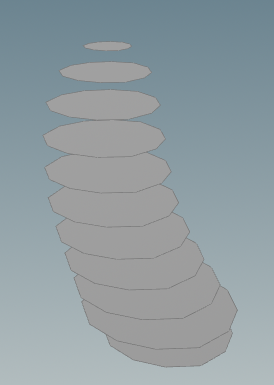
\includegraphics[width=\linewidth]{./figure/finger_scale_cross_section.png}}
\resizebox{4.3cm}{4.1cm}{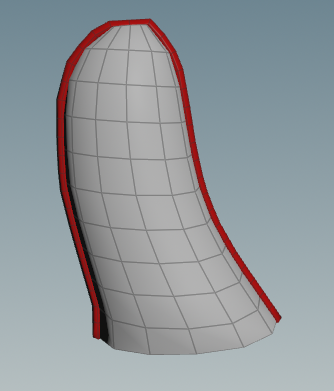
\includegraphics[width=\linewidth]{./figure/finger.png}}
\resizebox{4.3cm}{4.1cm}{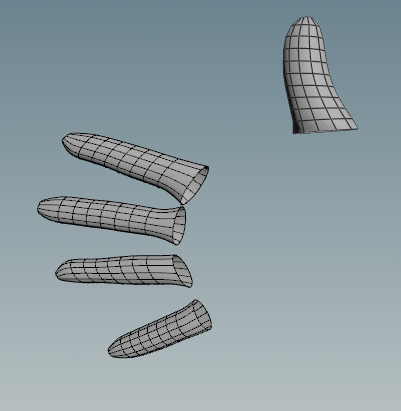
\includegraphics[width=\linewidth]{./figure/5fingers.png}}
\end{multicols}
\caption{a)direct deform from superellipsoid primitive, b)pre-process the superellipsoid's cross-sections c) deform the modified primitive and get the foot mesh d) e) f) same applies to the fingers}
\label{fig:footfinger}
\end{figure}


\noindent
Compare the following:\\
\begin{tabular}{ll}
 \verb'$conf_a$' &  $conf_a$ \\
 \verb'$\mathit{conf}_a$' & $\mathit{conf}_a$
\end{tabular}\\
See The \TeX book, p165.

The space after \eg, meaning ``for example'', should not be a
sentence-ending space. So \eg is correct, {\em e.g.} is not.  The provided
\verb'\eg' macro takes care of this.

When citing a multi-author paper, you may save space by using ``et alia'',
shortened to ``\etal'' (not ``{\em et.\ al.}'' as ``{\em et}'' is a complete word.)
However, use it only when there are three or more authors.  Thus, the
following is correct: ``
   Frobnication has been trendy lately.
   It was introduced by Alpher~\cite{Alpher02}, and subsequently developed by
   Alpher and Fotheringham-Smythe~\cite{Alpher03}, and Alpher \etal~\cite{Alpher04}.''

This is incorrect: ``... subsequently developed by Alpher \etal~\cite{Alpher03} ...''
because reference~\cite{Alpher03} has just two authors.  If you use the
\verb'\etal' macro provided, then you need not worry about double periods
when used at the end of a sentence as in Alpher \etal.

For this citation style, keep multiple citations in numerical (not
chronological) order, so prefer \cite{Alpher03,Alpher02,Authors12} to
\cite{Alpher02,Alpher03,Authors12}.



\section{Detail Generator} \label{detail_generator}
In order to add 3D details to 3D base mesh created from the primitive generator, we develop a detail generator consisting of a local shape creator and an image-based detail generator. In what follows, we first introduce the user interface of our developed detail generator in Subsection 5.1. Then we discuss the local shape creator and image-based detail generator in Subsections 5.2 and 5.3, respectively.

%------------------------------------------------------------------------

\section{Comparison and Future work}\label{comparison_and_future_work}

For now in the modelling stage of our system, all our control curves are creating smooth surfaces with C2 continuity, and the result template mesh looks pleasing as it is. In our future work, we will investigate the potentials of creases in more detailed character sculpting.
%-------------------------------------------------------------------------

\subsection{References}

List and number all bibliographical references in 9-point Times,
single-spaced, at the end of your paper. When referenced in the text,
enclose the citation number in square brackets, for
example~\cite{Authors12}.  Where appropriate, include the name(s) of
editors of referenced books.

\begin{table}
\begin{center}
\begin{tabular}{|l|c|}
\hline
Name & Performance \\
\hline\hline
A & OK\\
B & Bad \\
Ours & Great\\
\hline
\end{tabular}
\end{center}
\caption{An example for using tables.}
\end{table}

%-------------------------------------------------------------------------
\subsection{Illustrations, graphs, and photographs}

All graphics should be centered.  Please ensure that any point you wish to
make is resolvable in a printed copy of the paper.  Resize fonts in figures
to match the font in the body text, and choose line widths which render
effectively in print.  Many readers (and reviewers), even of an electronic
copy, will choose to print your paper in order to read it.  You cannot
insist that they do otherwise, and therefore must not assume that they can
zoom in to see tiny details on a graphic.

When placing figures in \LaTeX, it's almost always best to use
\verb+\includegraphics+, and to specify the  figure width as a multiple of
the line width as in the example below
{\small\begin{verbatim}
   \usepackage[dvips]{graphicx} ...
   \includegraphics[width=0.8\linewidth]
                   {myfile.eps}
\end{verbatim}
}


%-------------------------------------------------------------------------

{\small
\bibliographystyle{cvm}
\bibliography{cvmbib}
}


\end{document}
